\section*{Bài 3}

\begin{enumerate}[label=(\alph*)]
\item Chứng minh rằng: Tồn tại vô số cặp số nguyên $(m, n)$ sao cho $ma + nb = \gcd \big( a, b \big)$.
\item Cài đặt thuật toán Euclid để tìm UCLN của hai số nguyên $a$ và $b$.
\item Cài đặt thuật toán Euclid mở rộng để xác định giá trị $\big( m, n \big)$ sao cho: $\gcd \big( a, b \big) = ma + nb$.
\end{enumerate}

\addcontentsline{toc}{section}{Bài 3}

\centering
\textbf{\underline{Bài làm:}}
\justifying

(a) Với thuật toán Euclid mở rộng, ta tìm được một nghiệm $\big(m, n \big)$ thỏa mãn phương trình $ma + nb = \gcd \big(a, b \big)$ $\big( 1 \big)$.\\
Với $k \in \mathbb{Z}$, ta có: $ma + nb = ma + nb + kab - kab = a \big( m - kb \big) + b \big( n + ka \big)$.\\
Ta nhận thấy nếu $\big( m, n \big)$ là một nghiệm của phương trình $\big( 1 \big)$ thì $\big( m - kb, n + ka \big)$ cũng là một nghiệm của phương trình $\big( 1 \big)$. Vì có vô số giá trị $k \in \mathbb{Z}$ nên ta cũng có vô số cặp $\big( m - kb, n + ka \big)$ là nghiệm của phương trình $\big( 1 \big)$.\\
Vậy ta chứng minh được tồn tại vô số cặp số nguyên $\big(m, n \big)$ sao cho $ma + nb =  \gcd \big(a, b \big)$.

(b)

\textbf{Mã giả của thuật toán:}
\begin{algorithm}
\setstretch{1.15}
\renewcommand{\algorithmcfname}{Thuật toán}

\caption{Thuật toán Euclid để tìm UCLN}
\SetKwInOut{Input}{Đầu vào}\SetKwInOut{Output}{Đầu ra}
\SetAlgoNoEnd\SetAlgoNoLine%

\Input{2 số nguyên không âm $a, b$.}
\Output{Số nguyên không âm $d$ sao cho $d = \gcd \big( a, b \big)$.}
\While{$b \neq 0$}{
    $r \leftarrow a \textbf{ mod } b$\\
    $a \leftarrow b$\\
    $b \leftarrow r$
}
\Return $a$
\end{algorithm}

\textbf{Hiện thực thuật toán trên Maple:}

Ta định nghĩa thủ tục (procedure) $\mathtt{GCD} \big( x, y \big)$ như trong hình bên dưới. Sau đó, ta chạy thử thuật toán để tìm UCLN của các cặp số sau:
$$\big( 8, 0 \big), \big( 11, 0 \big), \big(13, 13 \big), \big( 37, 600 \big), \big( 20, 100 \big), \big( 624129, 2061517 \big)$$

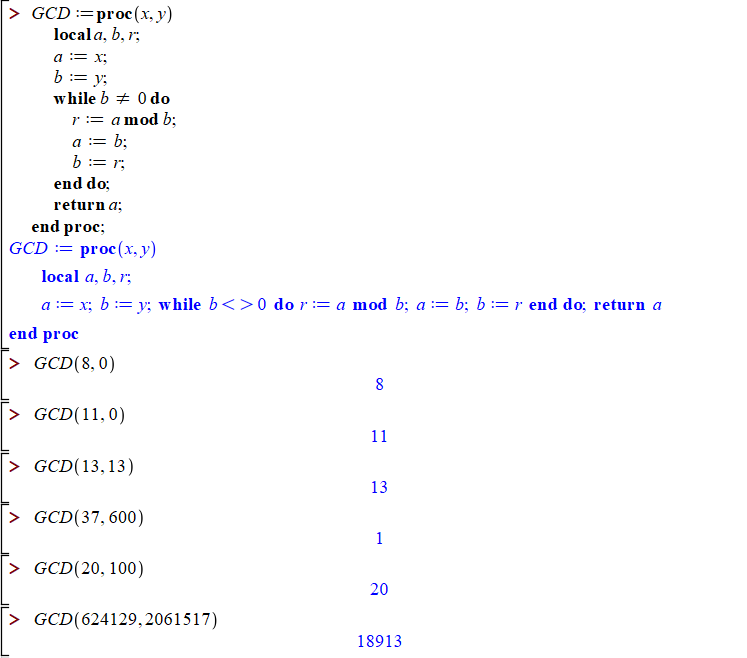
\includegraphics[width=1.0\textwidth]{bai3_GCD.png}

(c)

\textbf{Mã giả của thuật toán:}
\begin{algorithm}
\setstretch{1.15}
\renewcommand{\algorithmcfname}{Thuật toán}

\caption{Thuật toán Euclid mở rộng}
\SetKwInOut{Input}{Đầu vào}\SetKwInOut{Output}{Đầu ra}
\SetAlgoNoEnd\SetAlgoNoLine%

\Input{2 số nguyên không âm $a, b$.}
\Output{3 số nguyên $m, n, d$ sao cho $ma + nb = \gcd \big( a, b \big) = d$.}
$\big( m, n, d \big) \leftarrow \big( 1, 0, a \big)$\\
$\big( u_1, u_2, u_3 \big) \leftarrow \big( 0, 1, b \big)$\\
\While{$u_3 \neq 0$}{
    $\displaystyle q \leftarrow \left \lfloor{\frac{d}{u_3}}\right \rfloor $\\
    $\big( v_1, v_2, v_3 \big) \leftarrow \big( m, n, d \big) - q \big( u_1, u_2, u_3 \big)$\\
    $\big( m, n, d \big) \leftarrow \big( u_1, u_2, u_3 \big)$\\
    $\big( u_1, u_2, u_3 \big) \leftarrow \big( v_1, v_2, v_3 \big)$
}
\Return $m, n, d$
\end{algorithm}

\textbf{Hiện thực thuật toán trên Maple:}

Ta định nghĩa thủ tục (procedure) $\mathtt{ExtendedGCD} \big( a, b \big)$ như trong hình bên dưới. Sau đó, ta chạy thử thuật toán để tìm giá trị $m, n, d$ của các cặp số sau:
$$\big( 29, 8 \big), \big( 1398, 324 \big)$$.

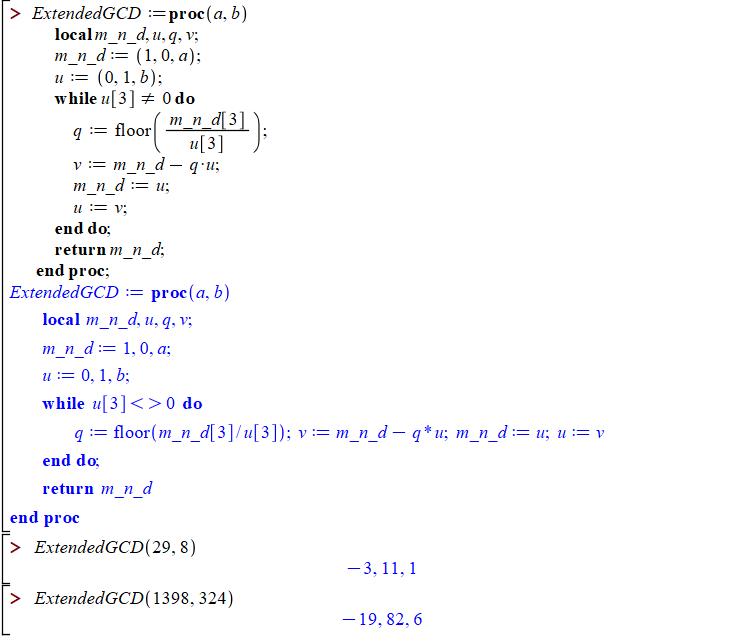
\includegraphics[width=1.0\textwidth]{bai3_extended_GCD.png}
	
\clearpage